  
\chapter{Results}
To test the software, the two stations were situated one outside the Electric and Electronic labs at Stellenbosch University and the other inside, with the UART giving the output as follows:
\definecolor{mygreen}{rgb}{0,0.6,0}
\definecolor{mygray}{rgb}{0.5,0.5,0.5}
\definecolor{mymauve}{rgb}{0.58,0,0.82}
\definecolor{terminalbgcolor}{HTML}{330033}
\definecolor{terminalrulecolor}{HTML}{000099}
\lstset{
	backgroundcolor=\color{terminalbgcolor},
	basicstyle=\color{white}\fontfamily{fvm}\footnotesize\selectfont,
	breakatwhitespace=false,  
	breaklines=true,
	captionpos=b,
	commentstyle=\color{mygreen},
	deletekeywords={...},
	escapeinside={\%*}{*)},
	extendedchars=true,
	frame=single,
	keepspaces=true,
	keywordstyle=\color{blue},
	%language=none,
	morekeywords={*,...},
	numbers=none,
	numbersep=5pt,
	framerule=2pt,
	numberstyle=\color{mygray}\tiny\selectfont,
	rulecolor=\color{terminalrulecolor},
	showspaces=false,
	showstringspaces=false,
	showtabs=false,
	stepnumber=2,
	stringstyle=\color{mymauve},
	tabsize=2
}
\begin{lstlisting}
Bytes received: 80
SATELLITE time: 2023/5/16-21:55:57 Location: -33.9286628330, 18.8670256670 CO2:  +469.00,
MassConcentrationPm1p0:  +3.60,MassConcentrationPm2p5: 3.80,MassConcentrationPm4p0: 3.80,
MassConcentrationPm10p0: 3.80,AmbientHumidity: 86.72,AmbientTemperature: 10.62C,
VocIndex: 19.00,NoxIndex: 1.00
\end{lstlisting}
This shows the received contents from the satellite station, as well as the size of the bytes received. This confirms the transfer system working as expected. With this confirmed, the next test was to see if the WiFi download server was working on the base station and if the data has been written to the SD card.




%First say what you are looking at. Then say what yo get from figure
%now given this what does it tell you
%for each table and figure

\vspace{-2em}
\section{Particulate Matter}
\vspace{-2em}
%\begin{figure}[!htb]
%	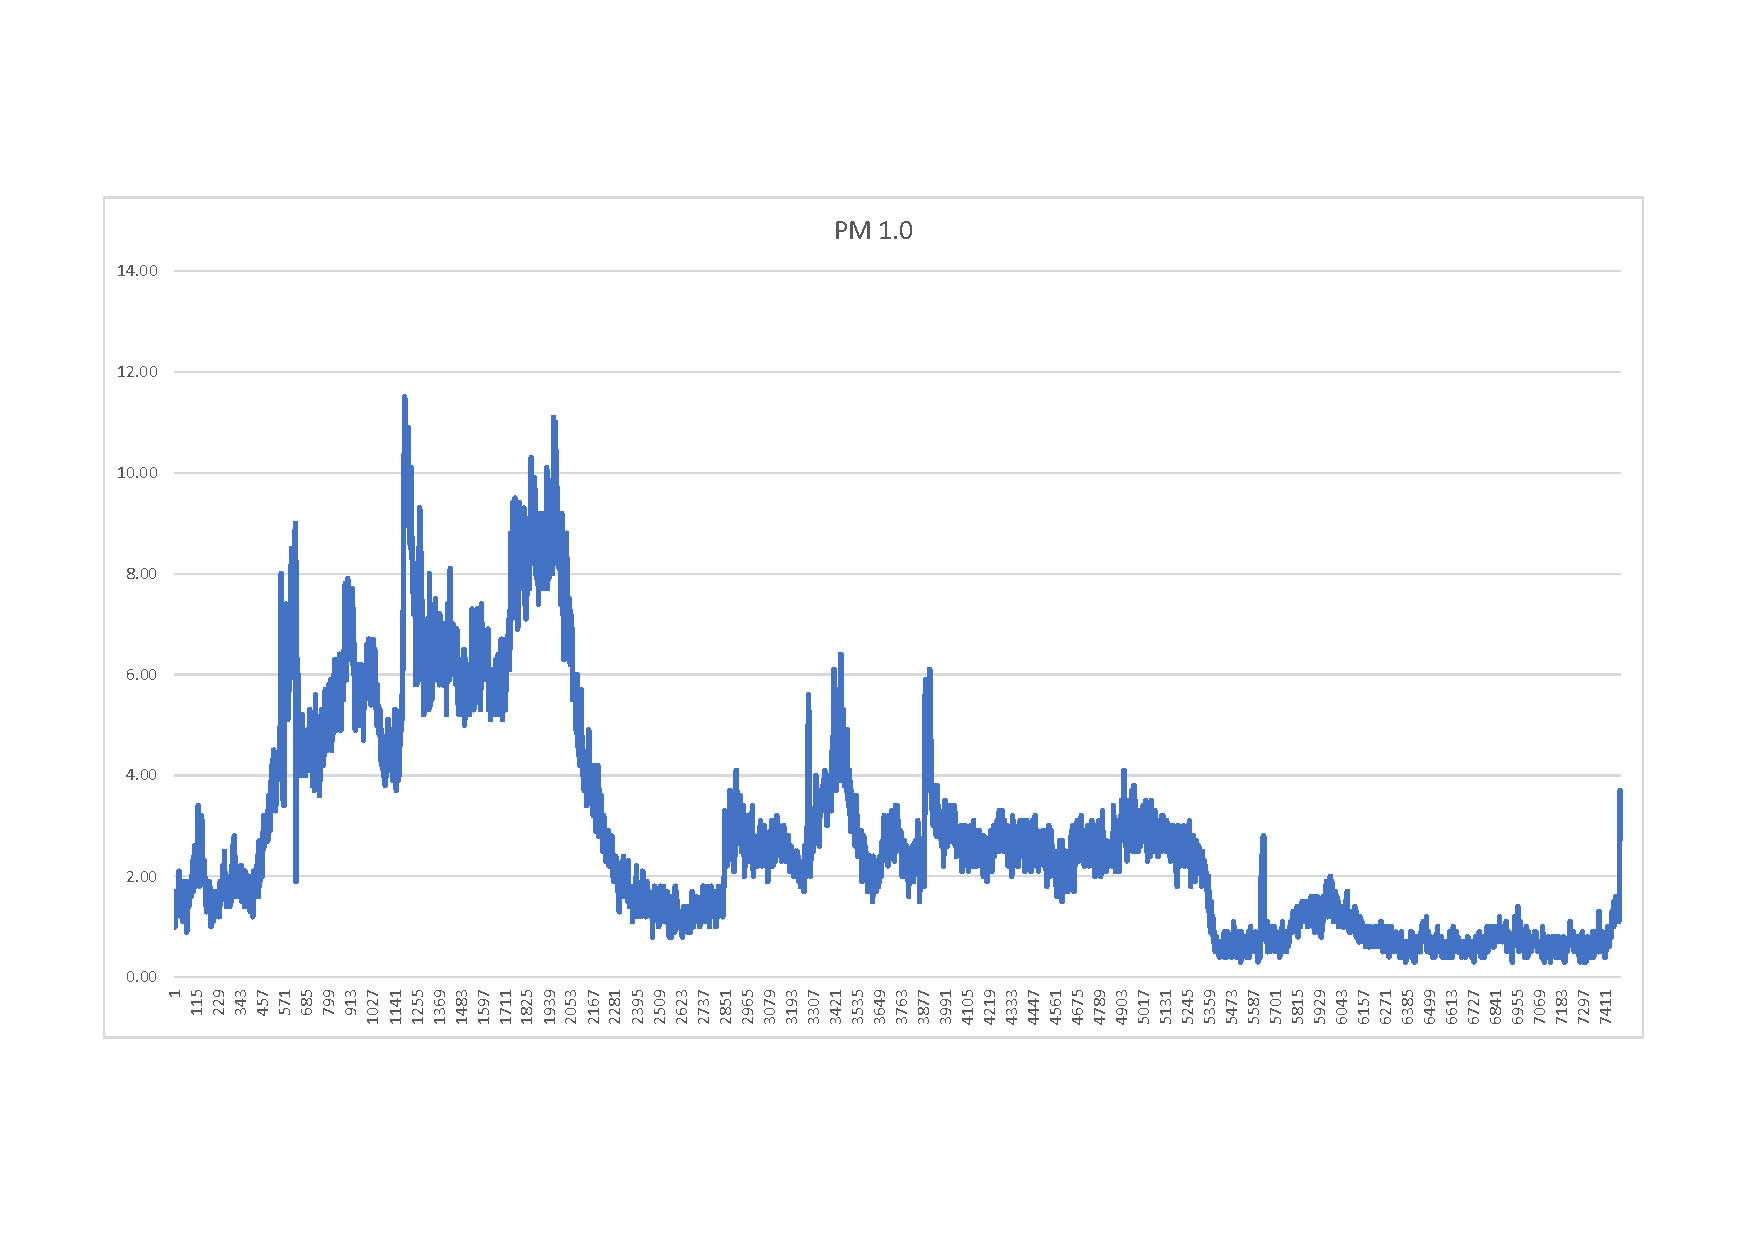
\includegraphics[width=0.45\textwidth, height = 10em]{body/fig/PM0.1.pdf}%
%	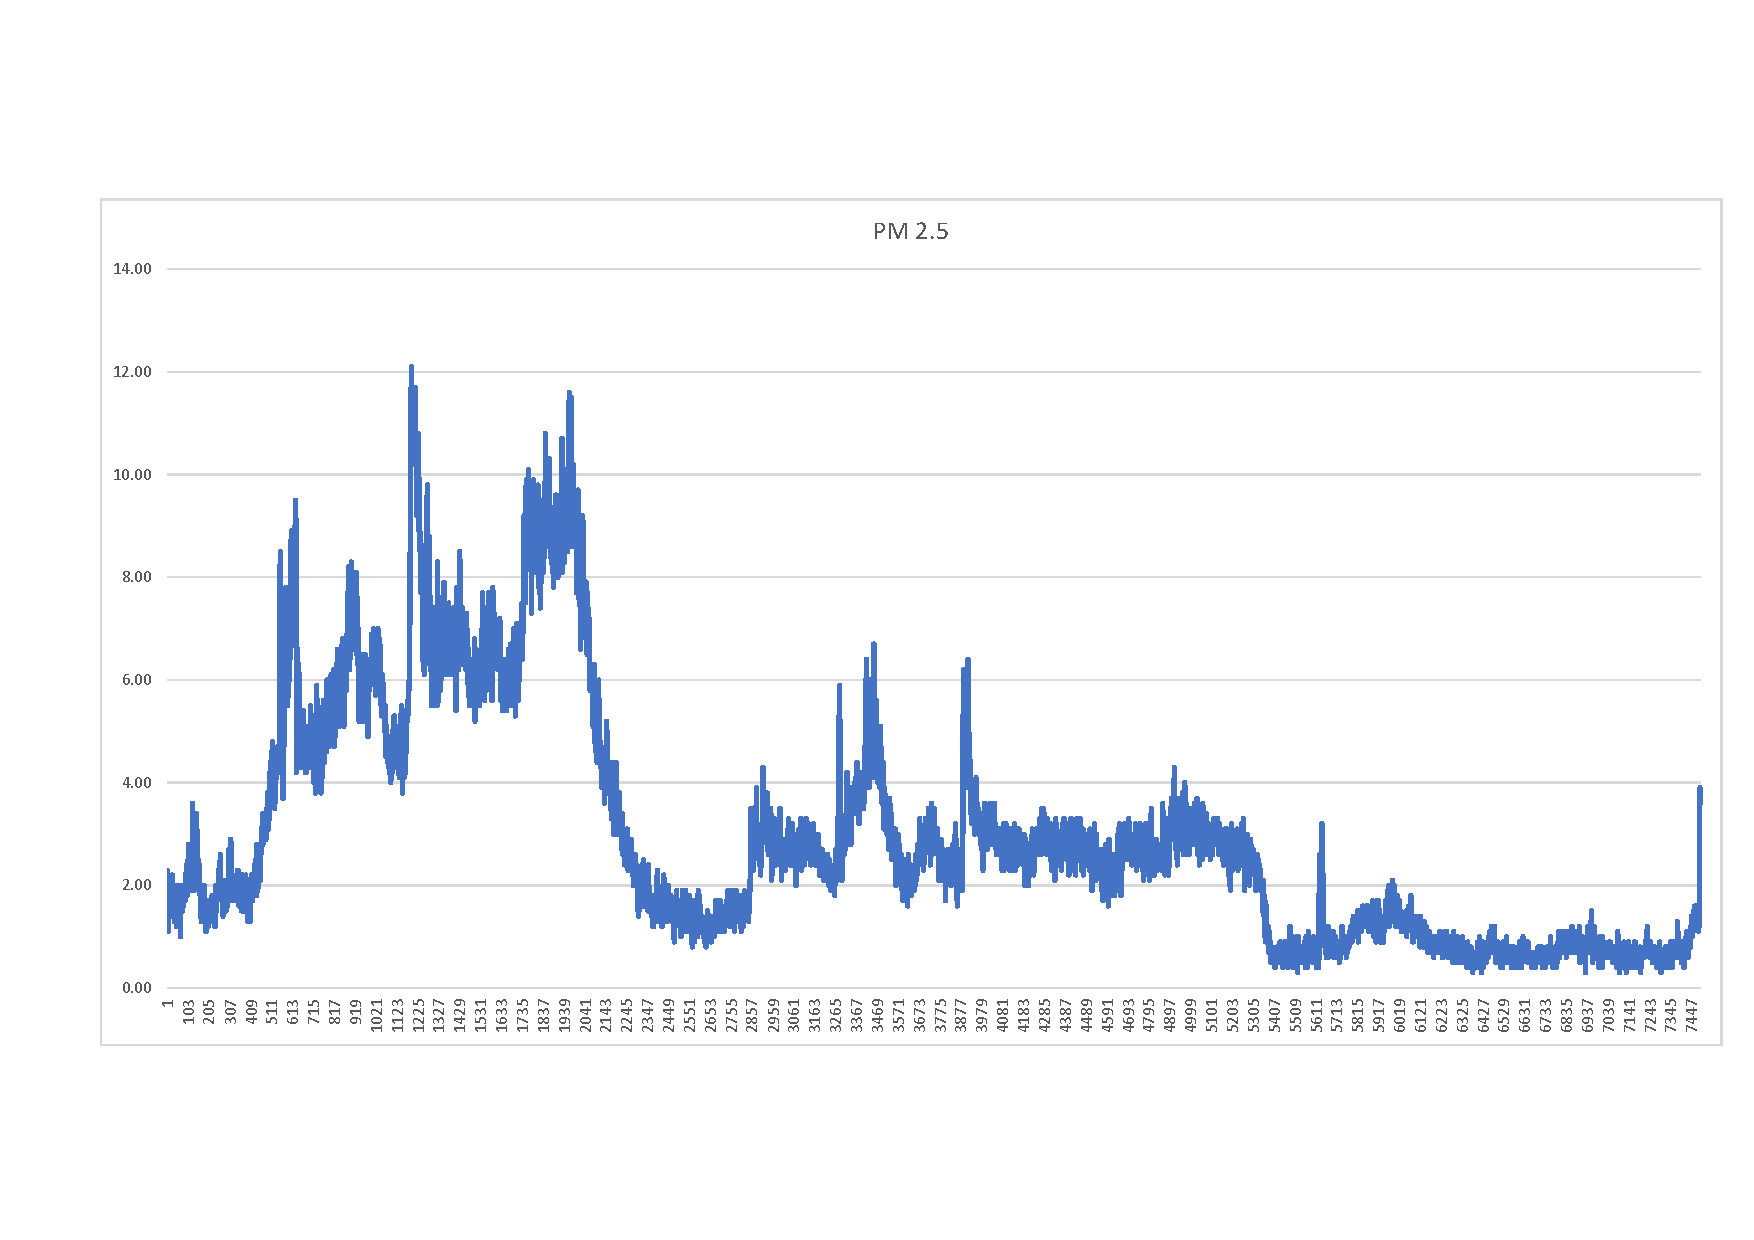
\includegraphics[width=0.45\textwidth, height = 10em]{body/fig/PM2.5.pdf}%
%	\caption{PM 1.0 (left) and PM 2.5 (right)}
%	\label{ACEM1}
%	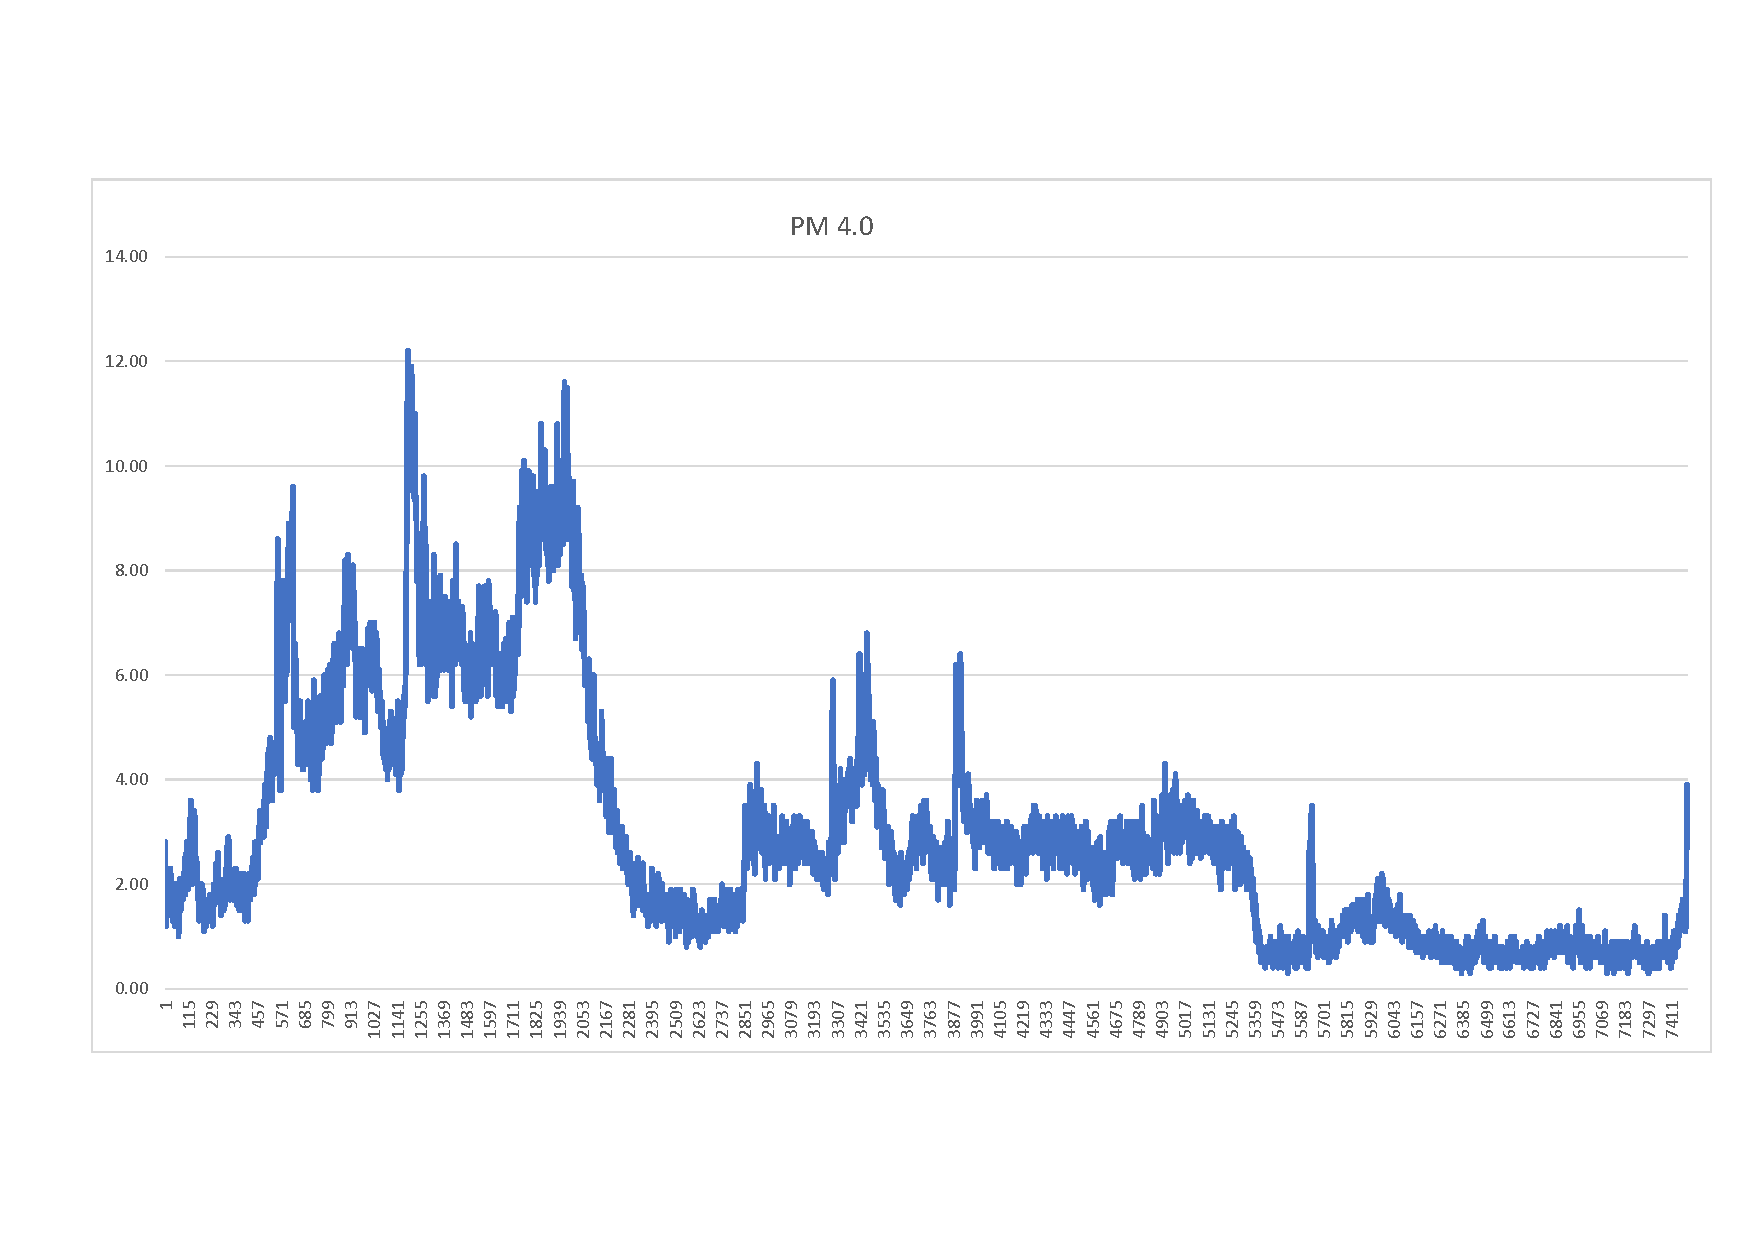
\includegraphics[width=0.45\textwidth, height = 10em]{body/fig/PM4.pdf}%
%	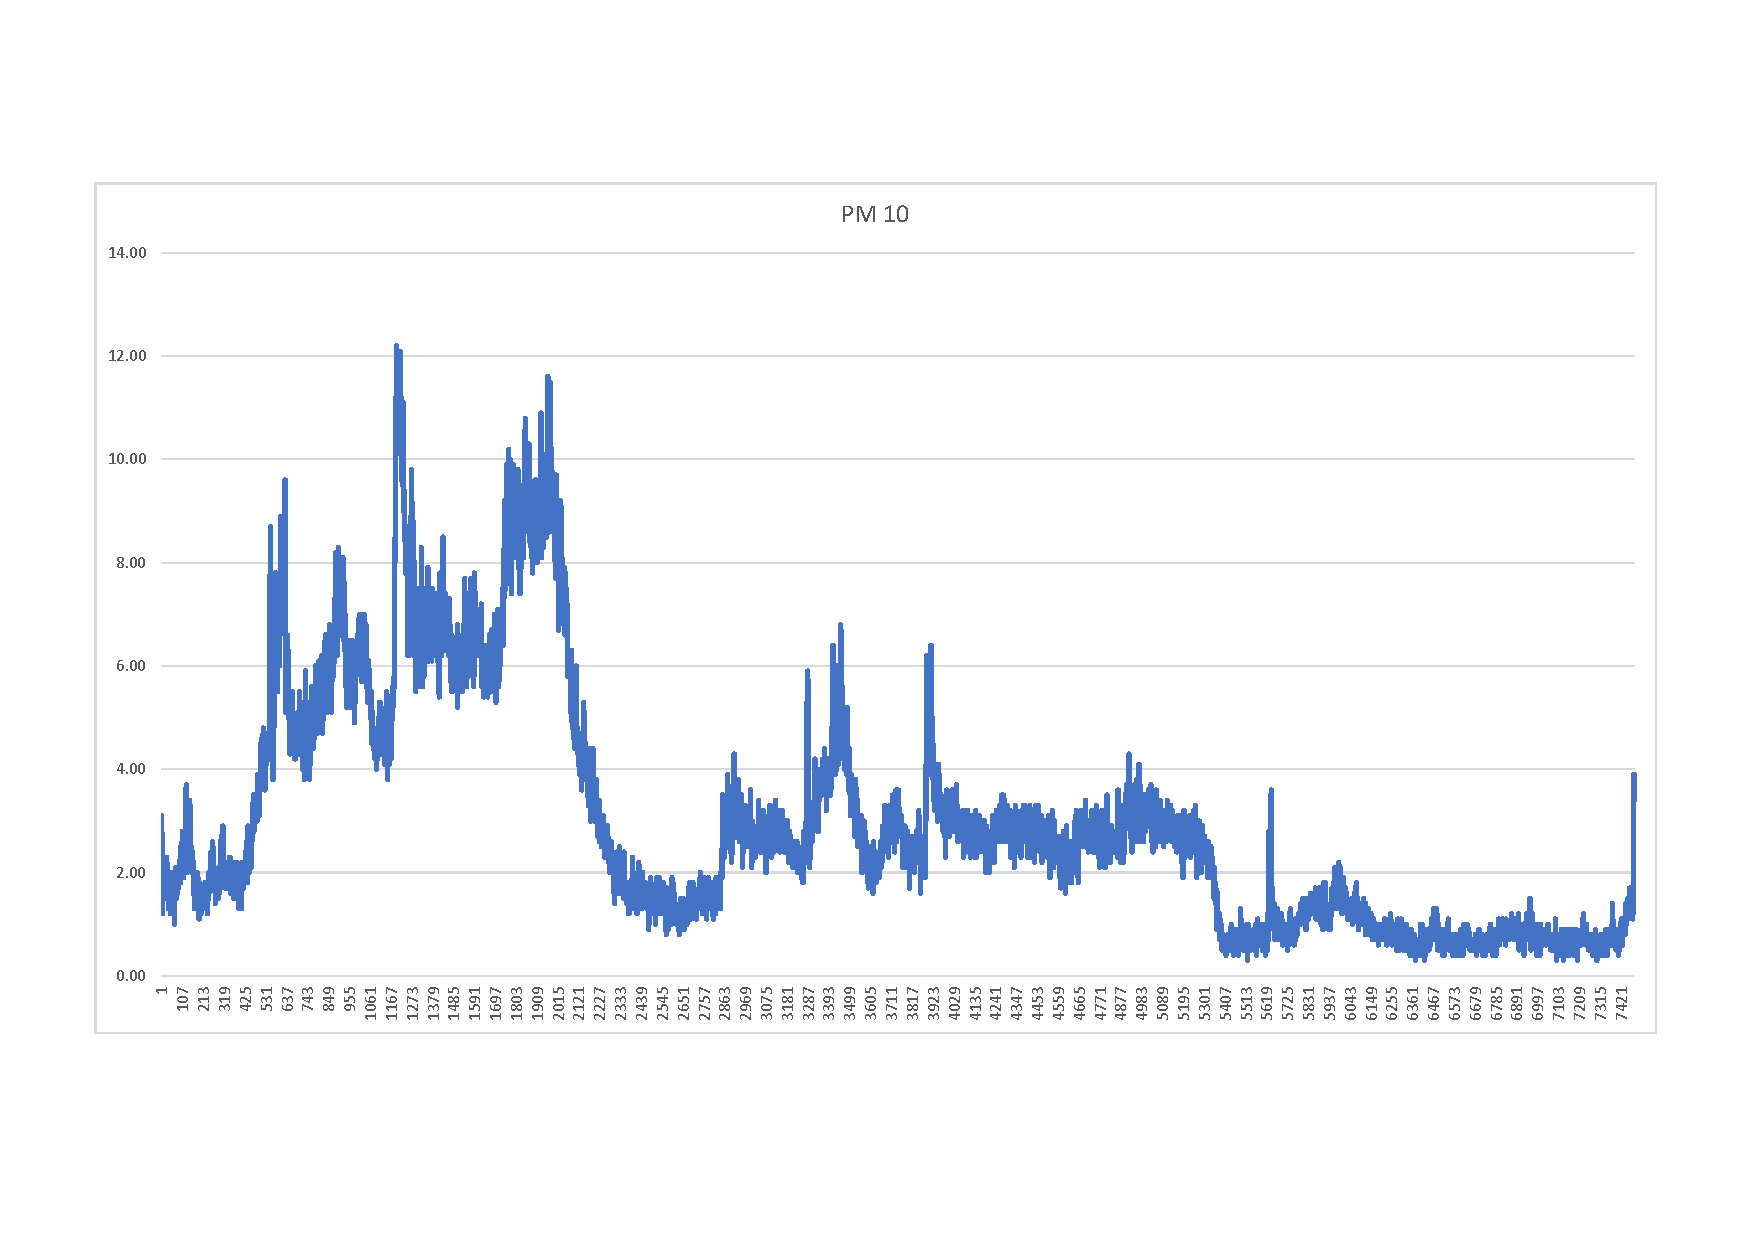
\includegraphics[width=0.45\textwidth, height = 10em]{body/fig/PM10.pdf}%
%	\captionof{figure}{PM 4.0 (left) and PM 10 (right)}
%	\label{ACEM2}
%\end{figure}
\begin{figure}[!htb]
	\centering
	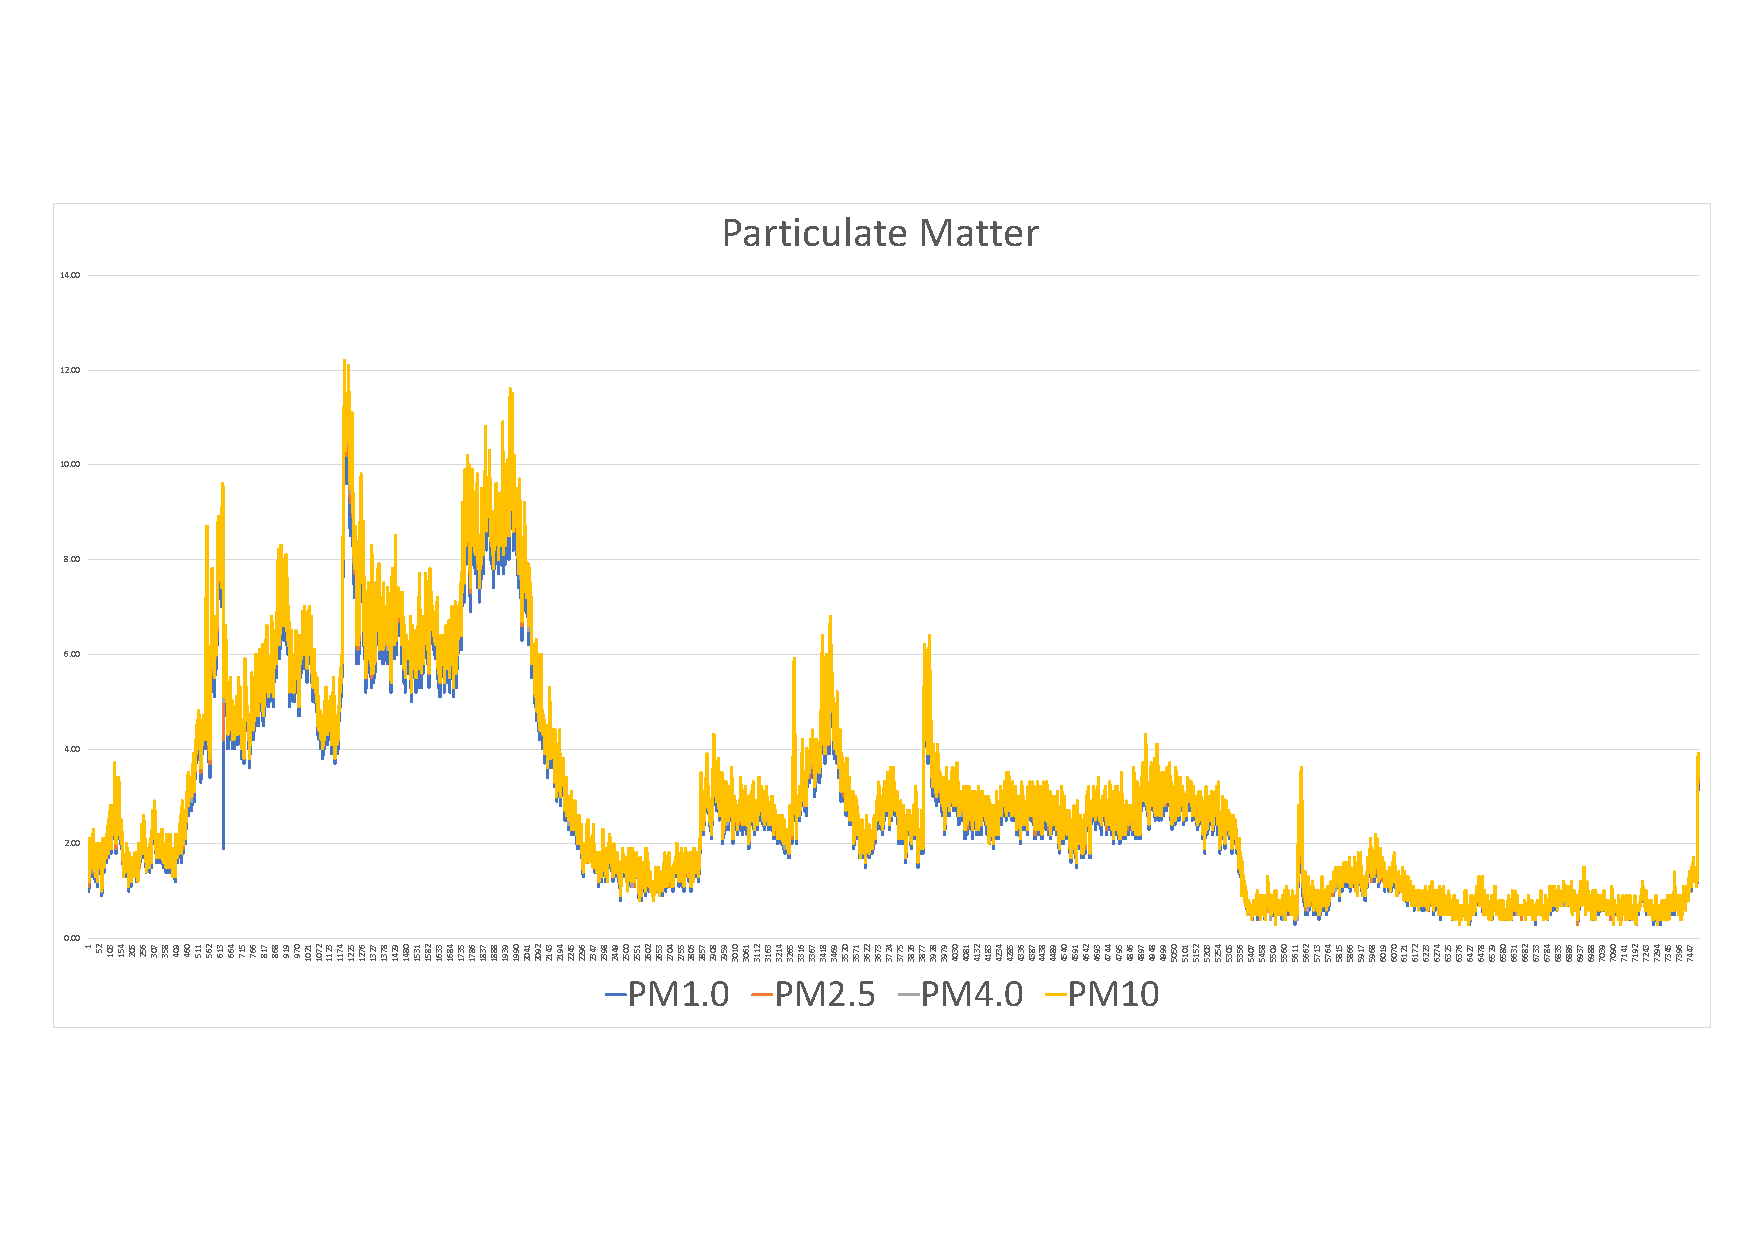
\includegraphics[width=0.9\linewidth]{body/fig/PMall.pdf}
	\caption{Particulate Matter graph of 7000 data points at all concentrations measured.}
	\label{fig:PMall}
\end{figure}

\noindent
The correlation between all of the different sizes of particulate matter concentrations is rather high, as can be seen from Figure~\ref{fig:PMall}, This means we could conceivably only use the PM 2.5 reading as is the norm. The rough timing of the chart is late afternoon to next day, with the elevated period in the middle representing the evening and sleep.


\begin{figure}[!htb]
	\centering
	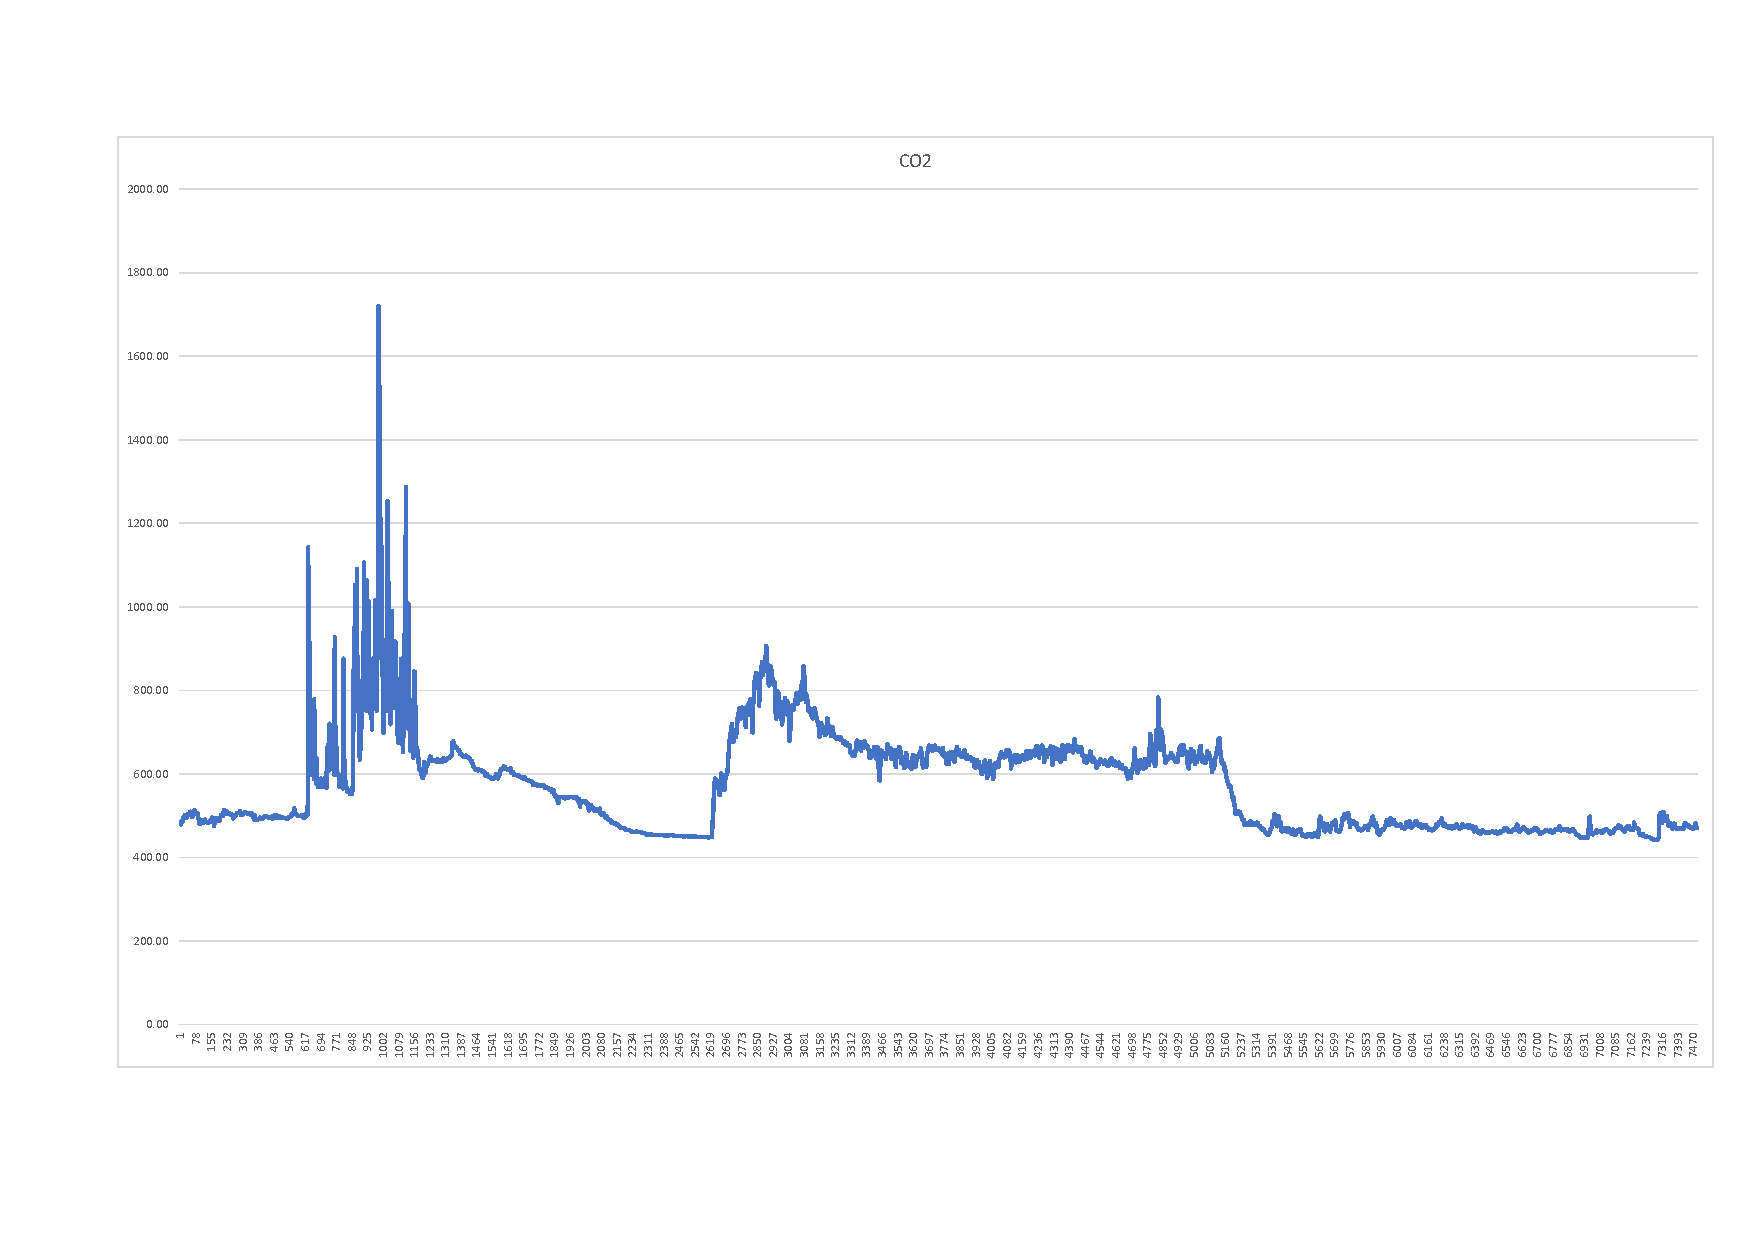
\includegraphics[width=0.7\linewidth]{body/fig/CO2}
	\caption{CO2 measurements}
	\label{fig:co2}
\end{figure}


%\begin{figure}[!htb]
%	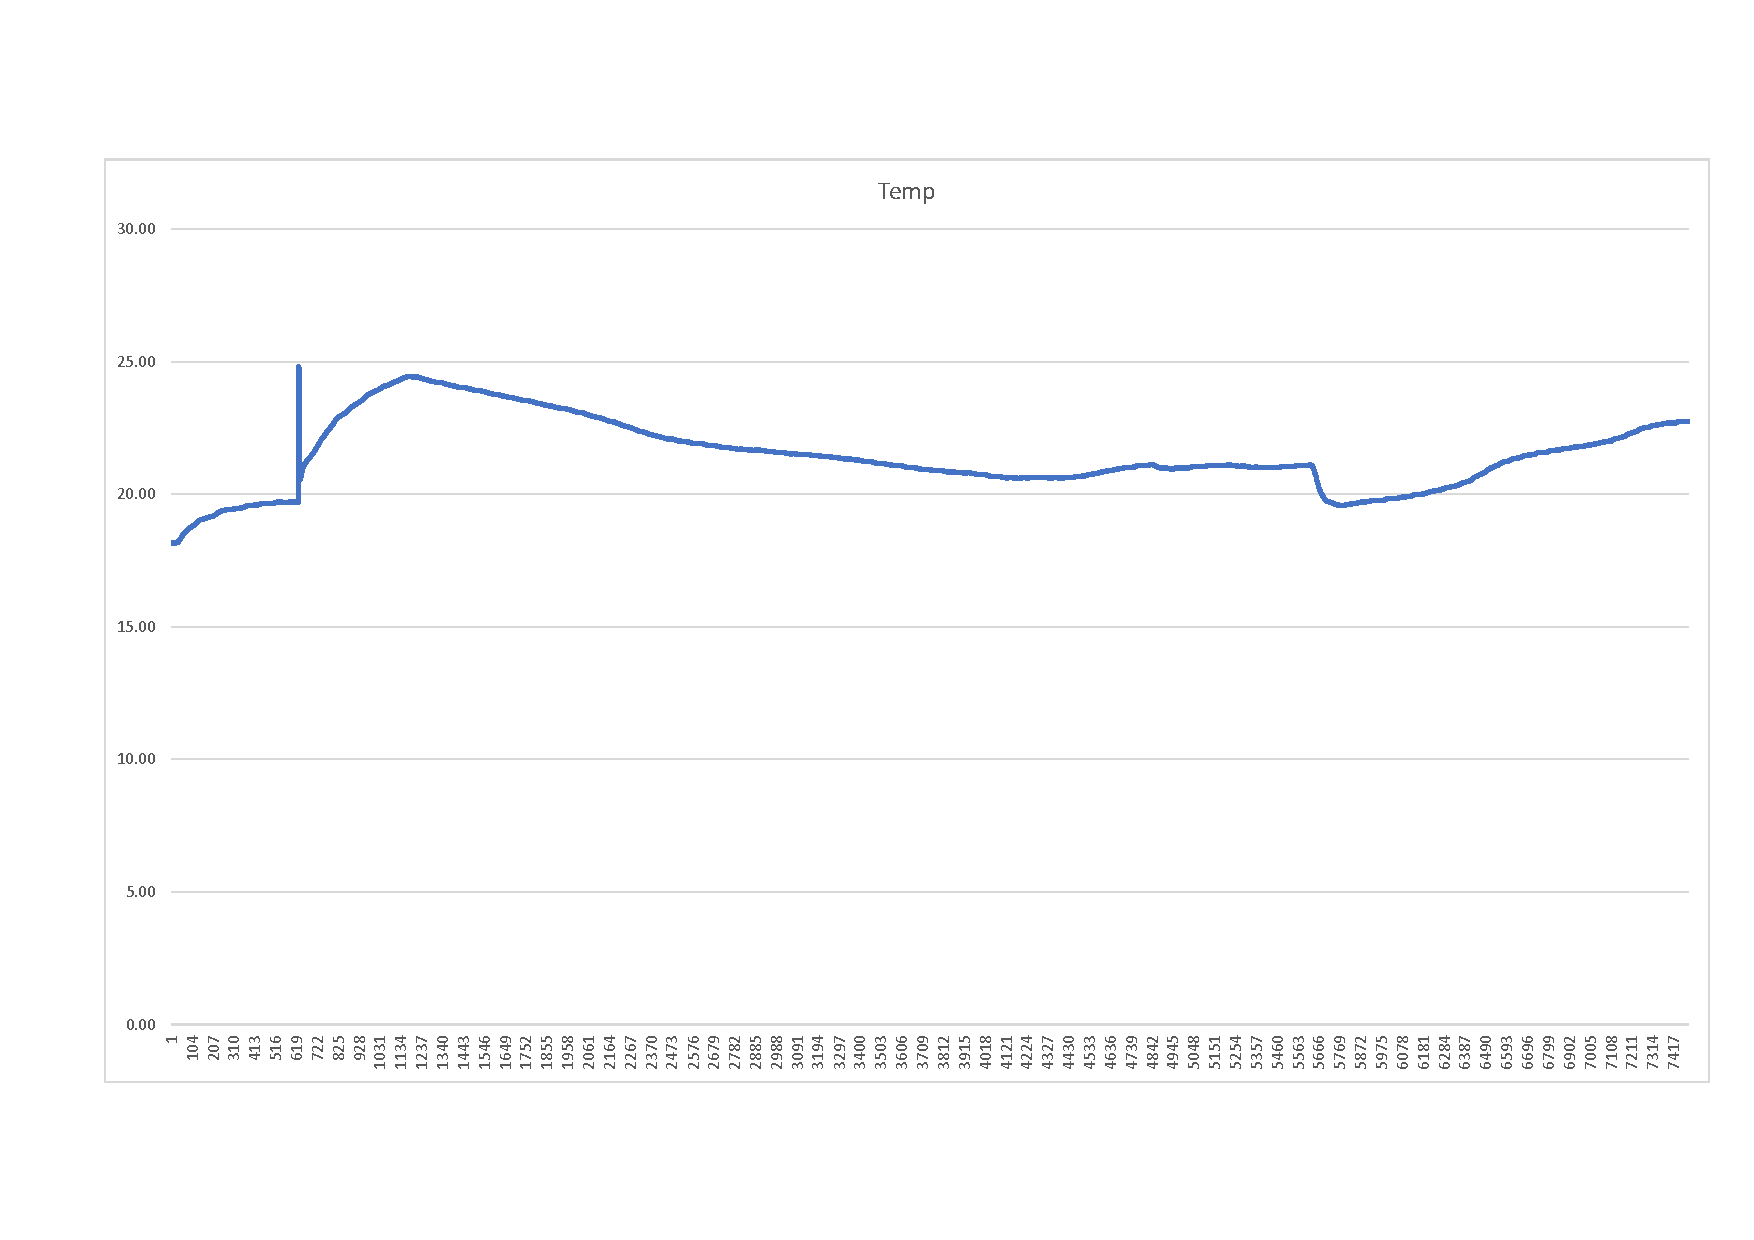
\includegraphics[width=0.5\textwidth]{body/fig/Temp.pdf}%
%	\caption{Temperature}
%	\label{fig:temp}
%	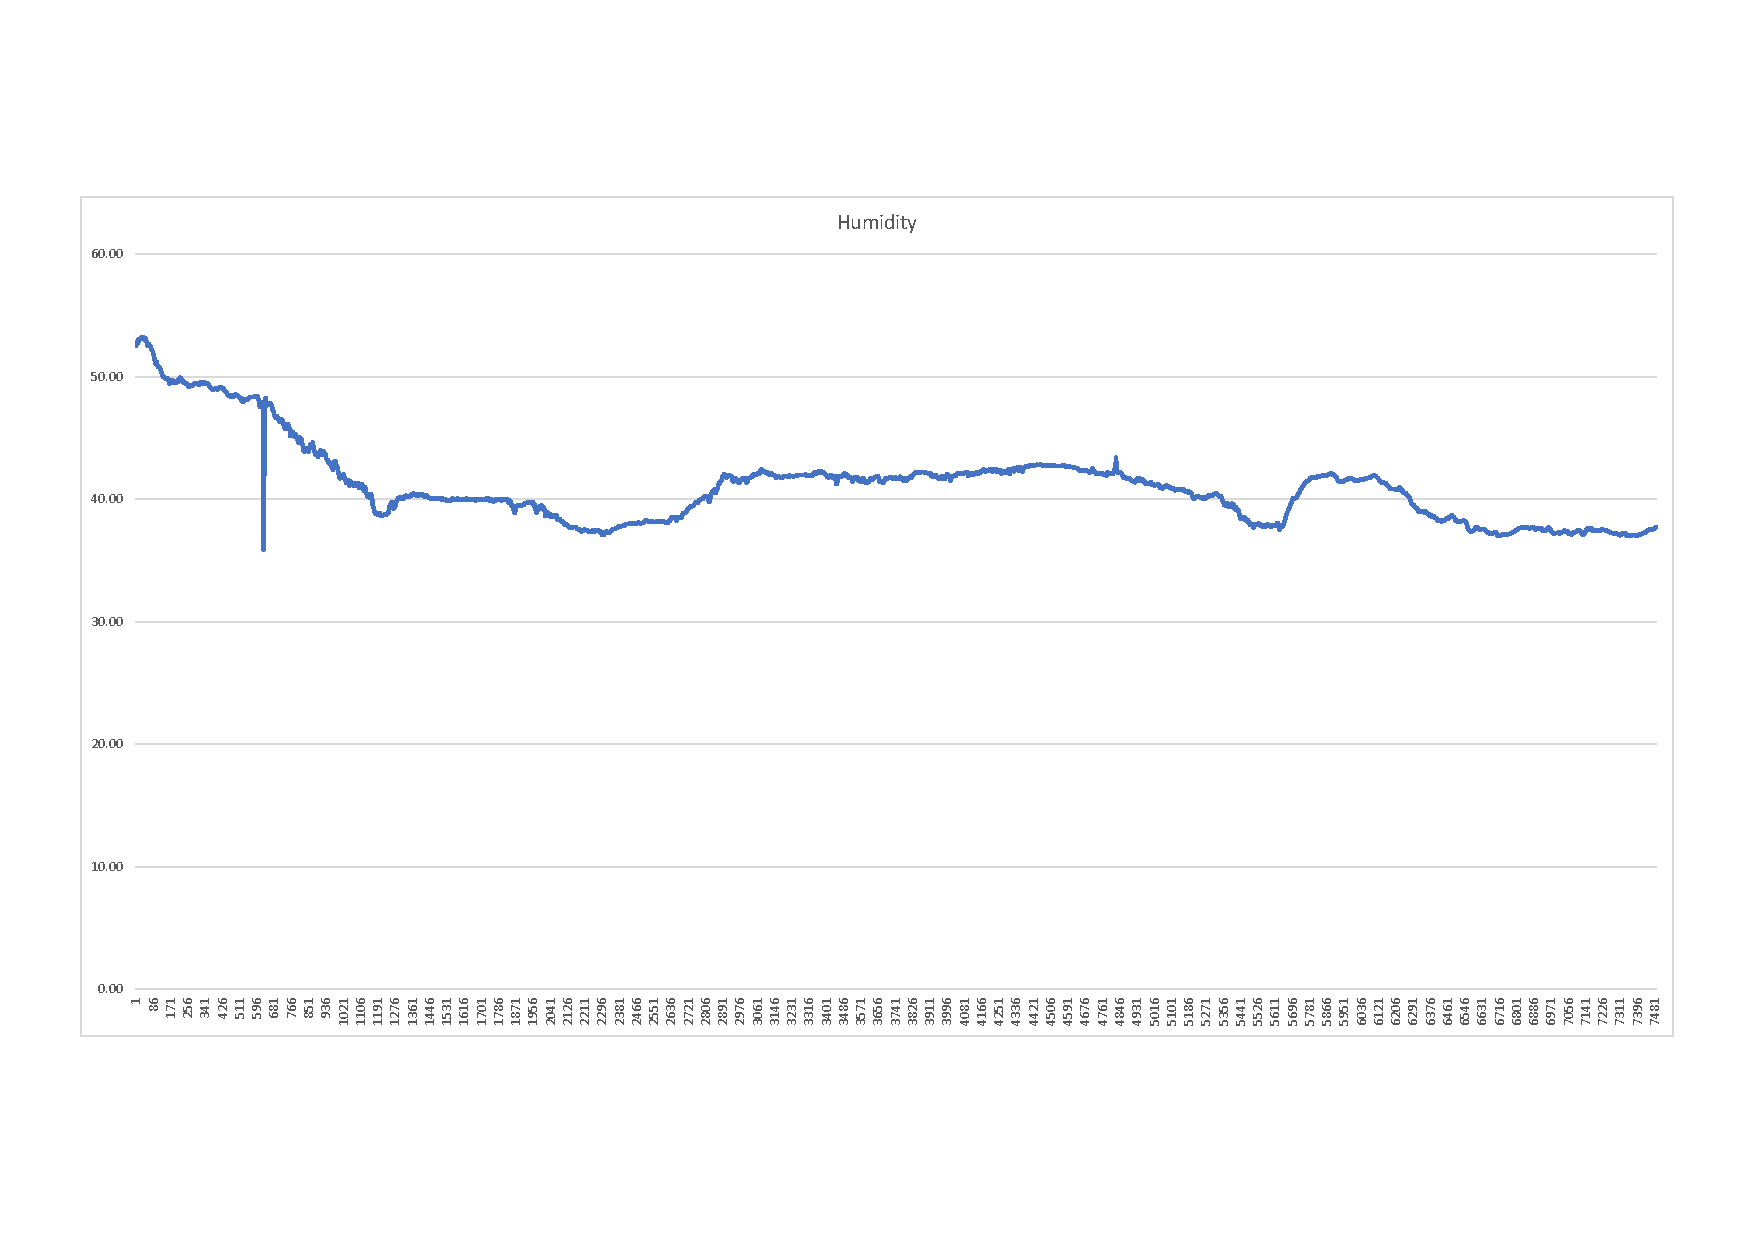
\includegraphics[width=0.5\textwidth]{body/fig/hum.pdf}%
%	\captionof{figure}{Humidity}
%	\label{fig:hum}
%\end{figure}
\begin{figure}[!htb]
	\minipage{0.45\textwidth}%
	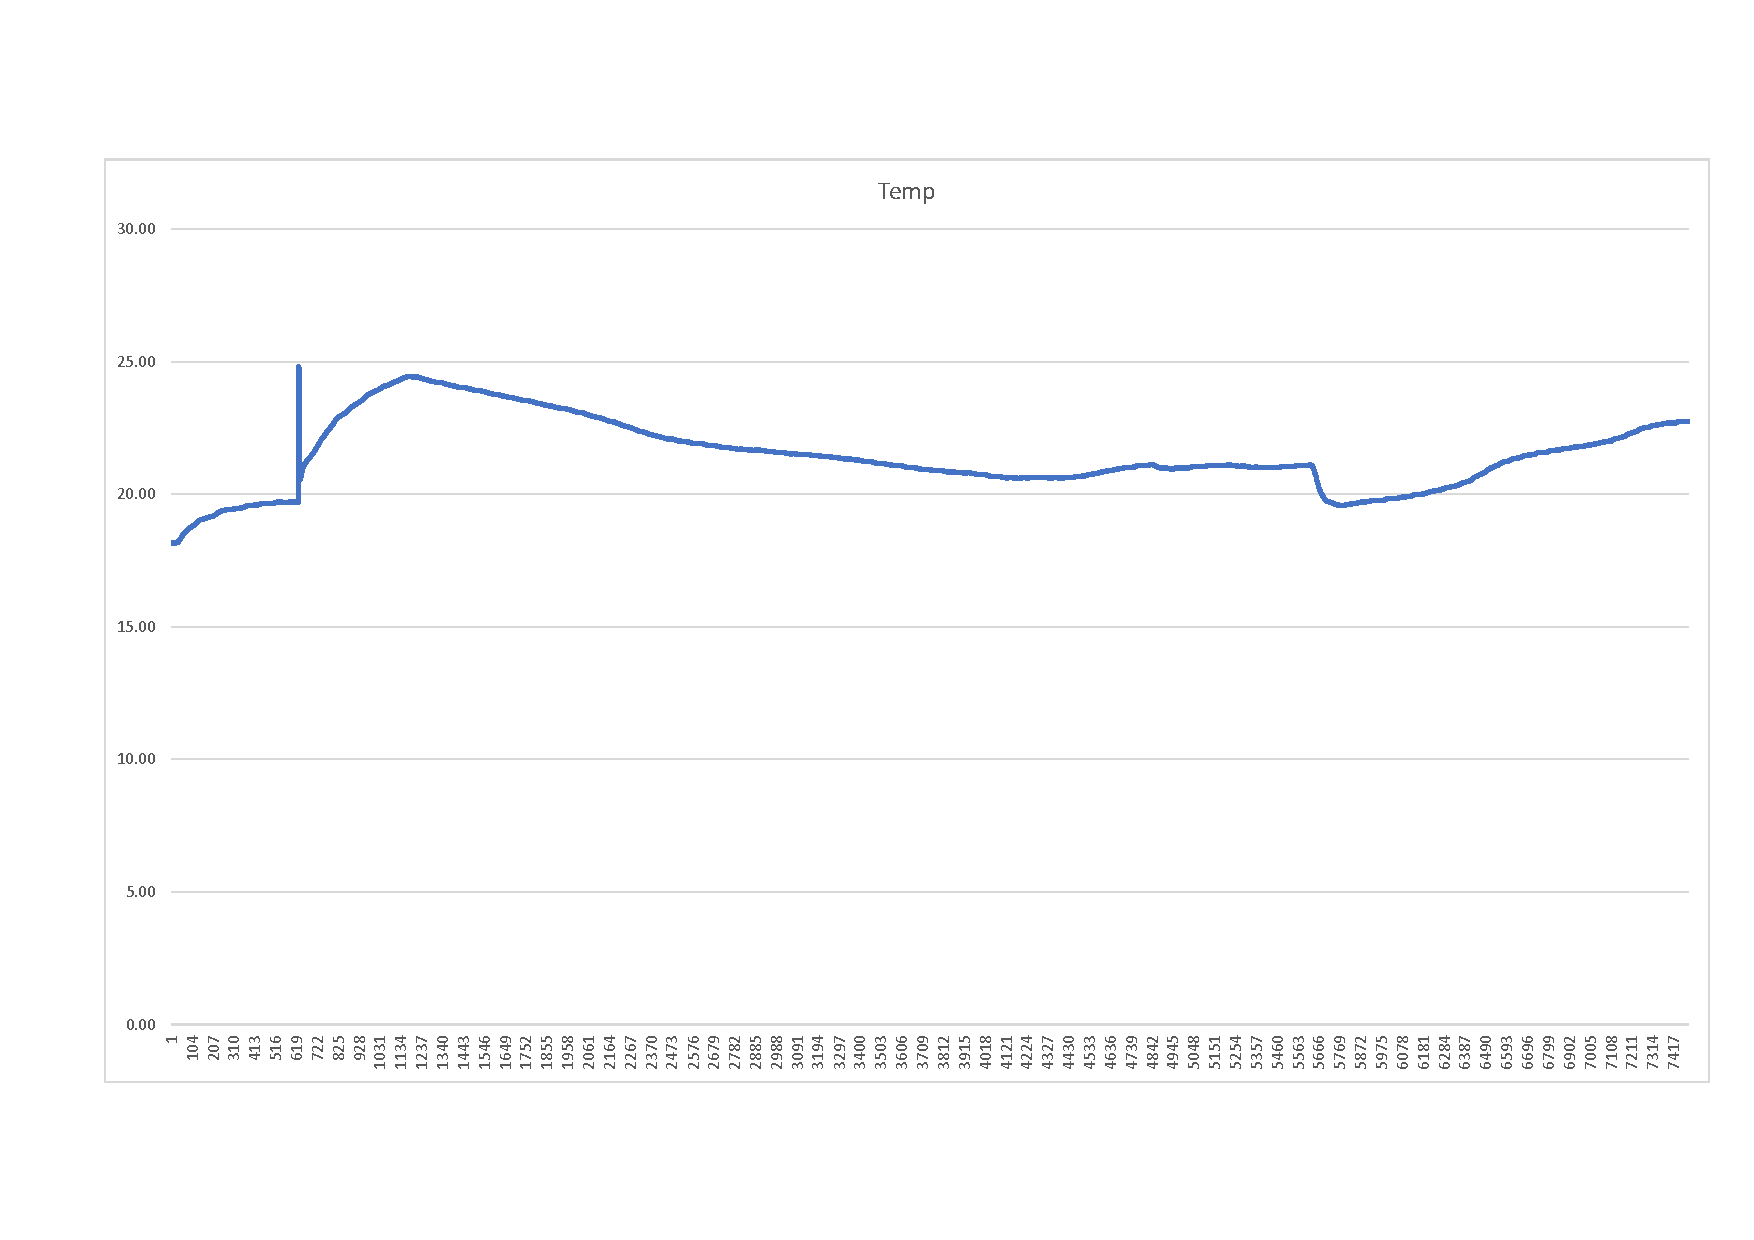
\includegraphics[width=\textwidth]{body/fig/Temp.pdf}%
\caption{Temperature}
\label{fig:temp}
	\endminipage\hfill
	\minipage{0.45\textwidth}%
	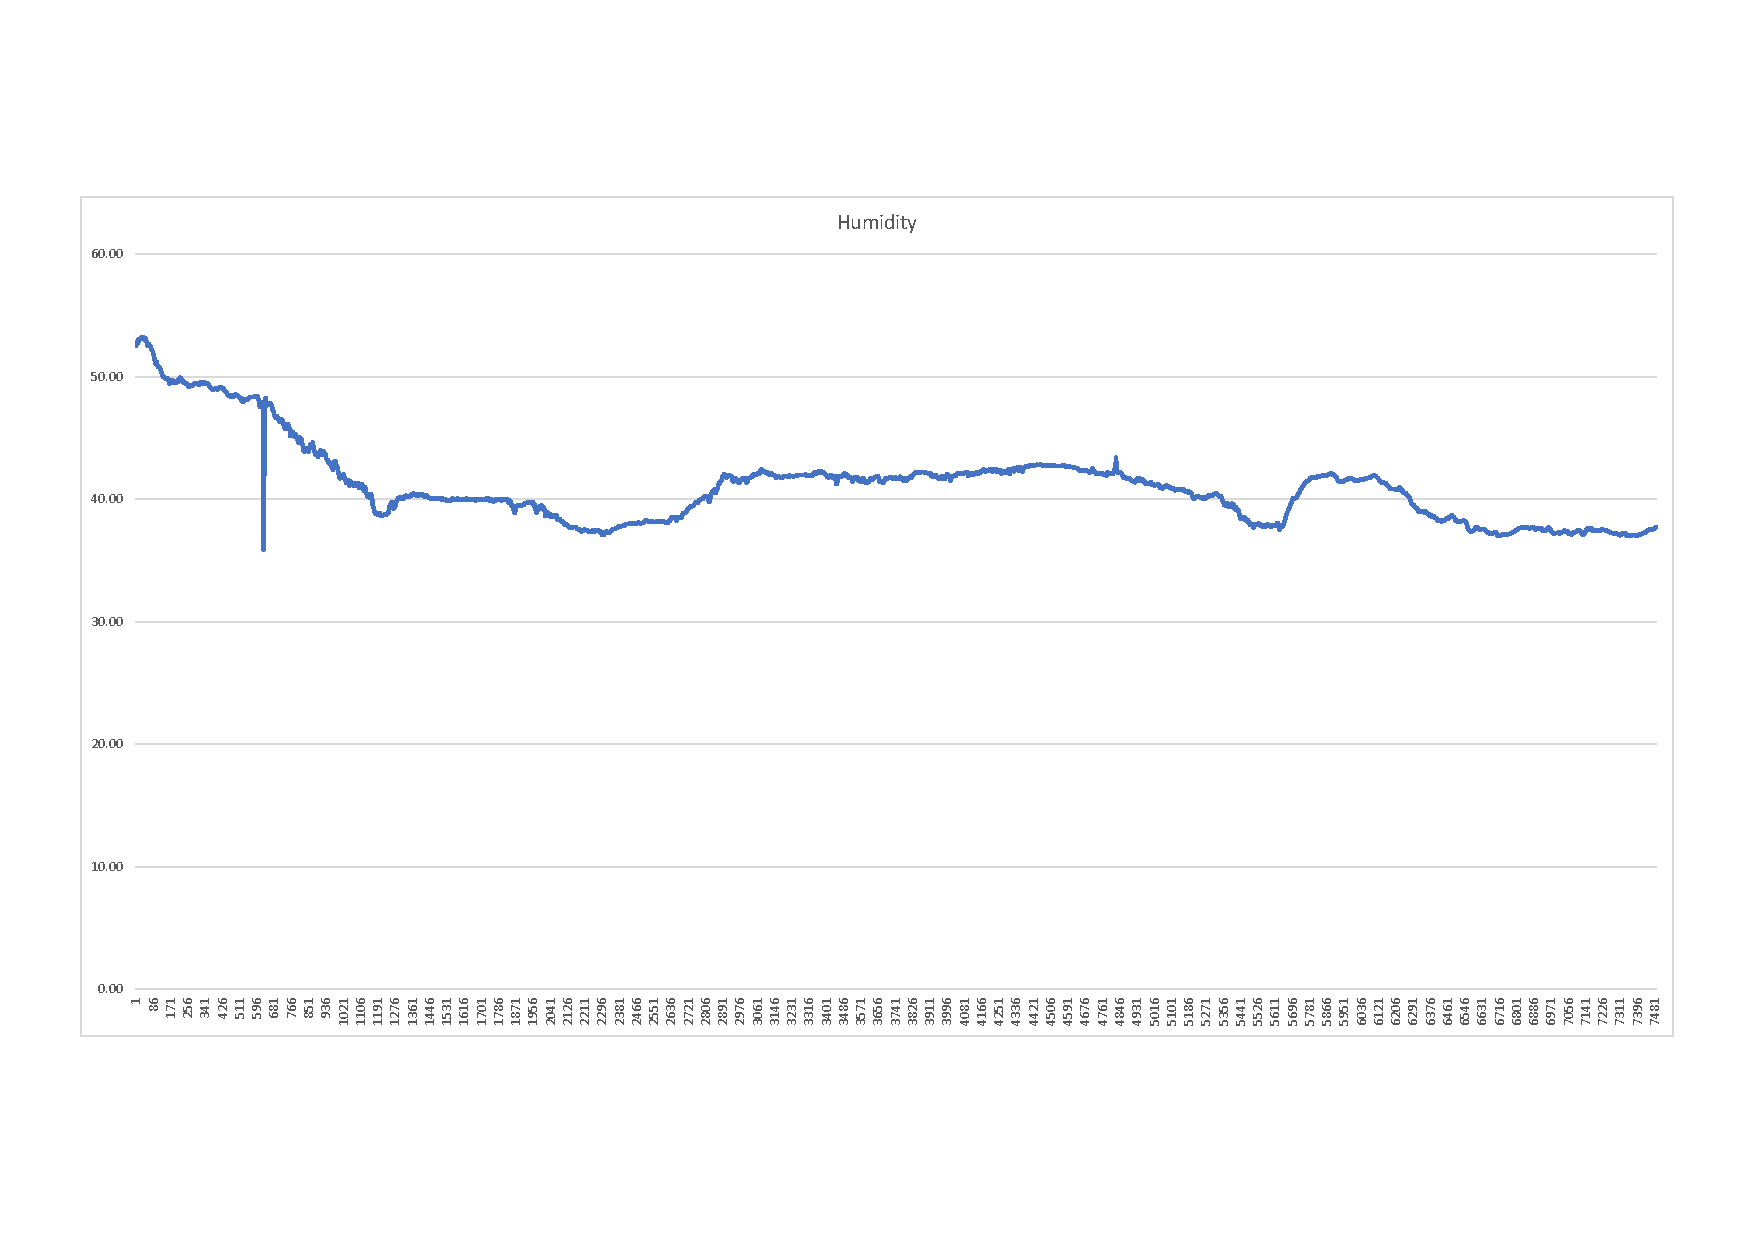
\includegraphics[width=\textwidth]{body/fig/hum.pdf}%
\captionof{figure}{Humidity}
\label{fig:hum}
	\endminipage\hfill
	
	%\text{Charts provided by \cite{2007Comparison}}
\end{figure}


%\begin{figure}[!htb]
%	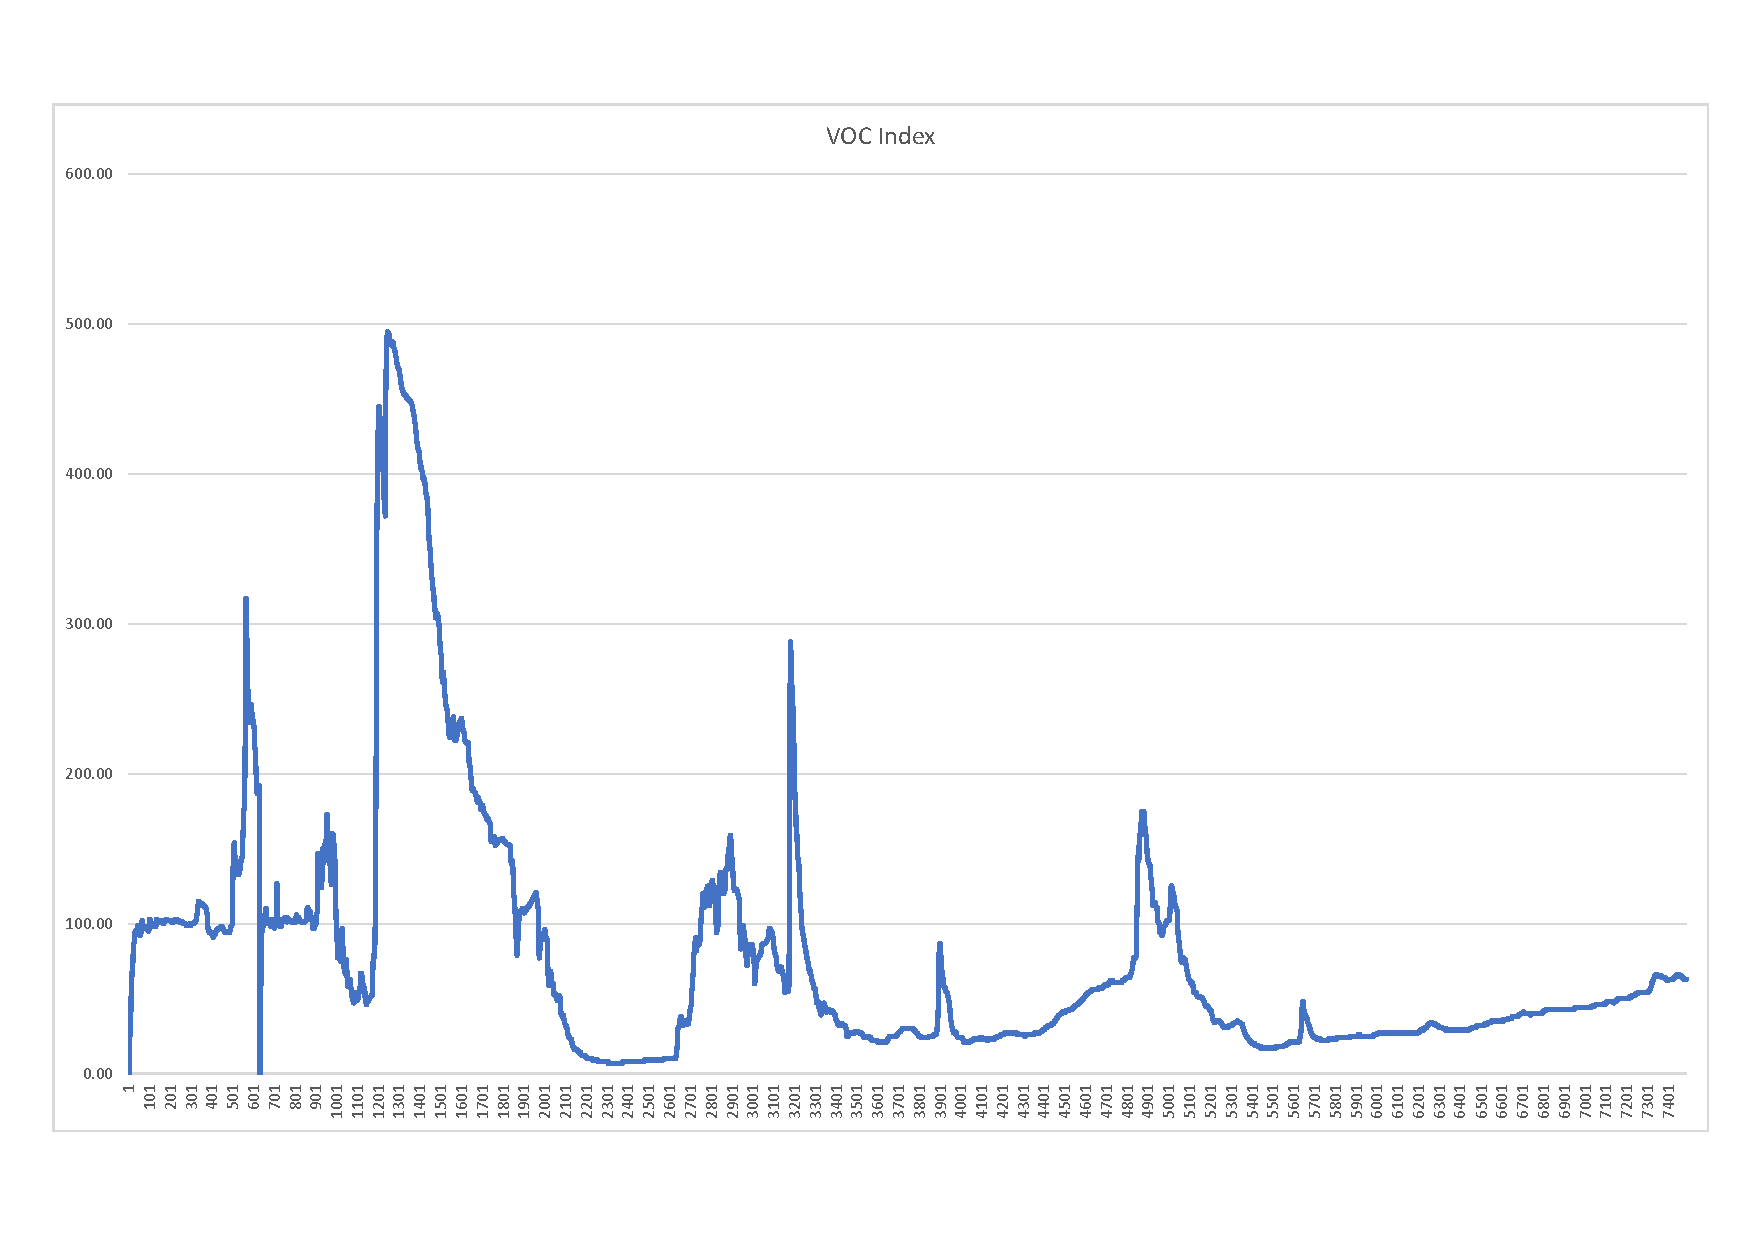
\includegraphics[width=0.5\textwidth]{body/fig/VOC.pdf}%
%	\caption{Temperature}
%	\label{fig:voc}
%	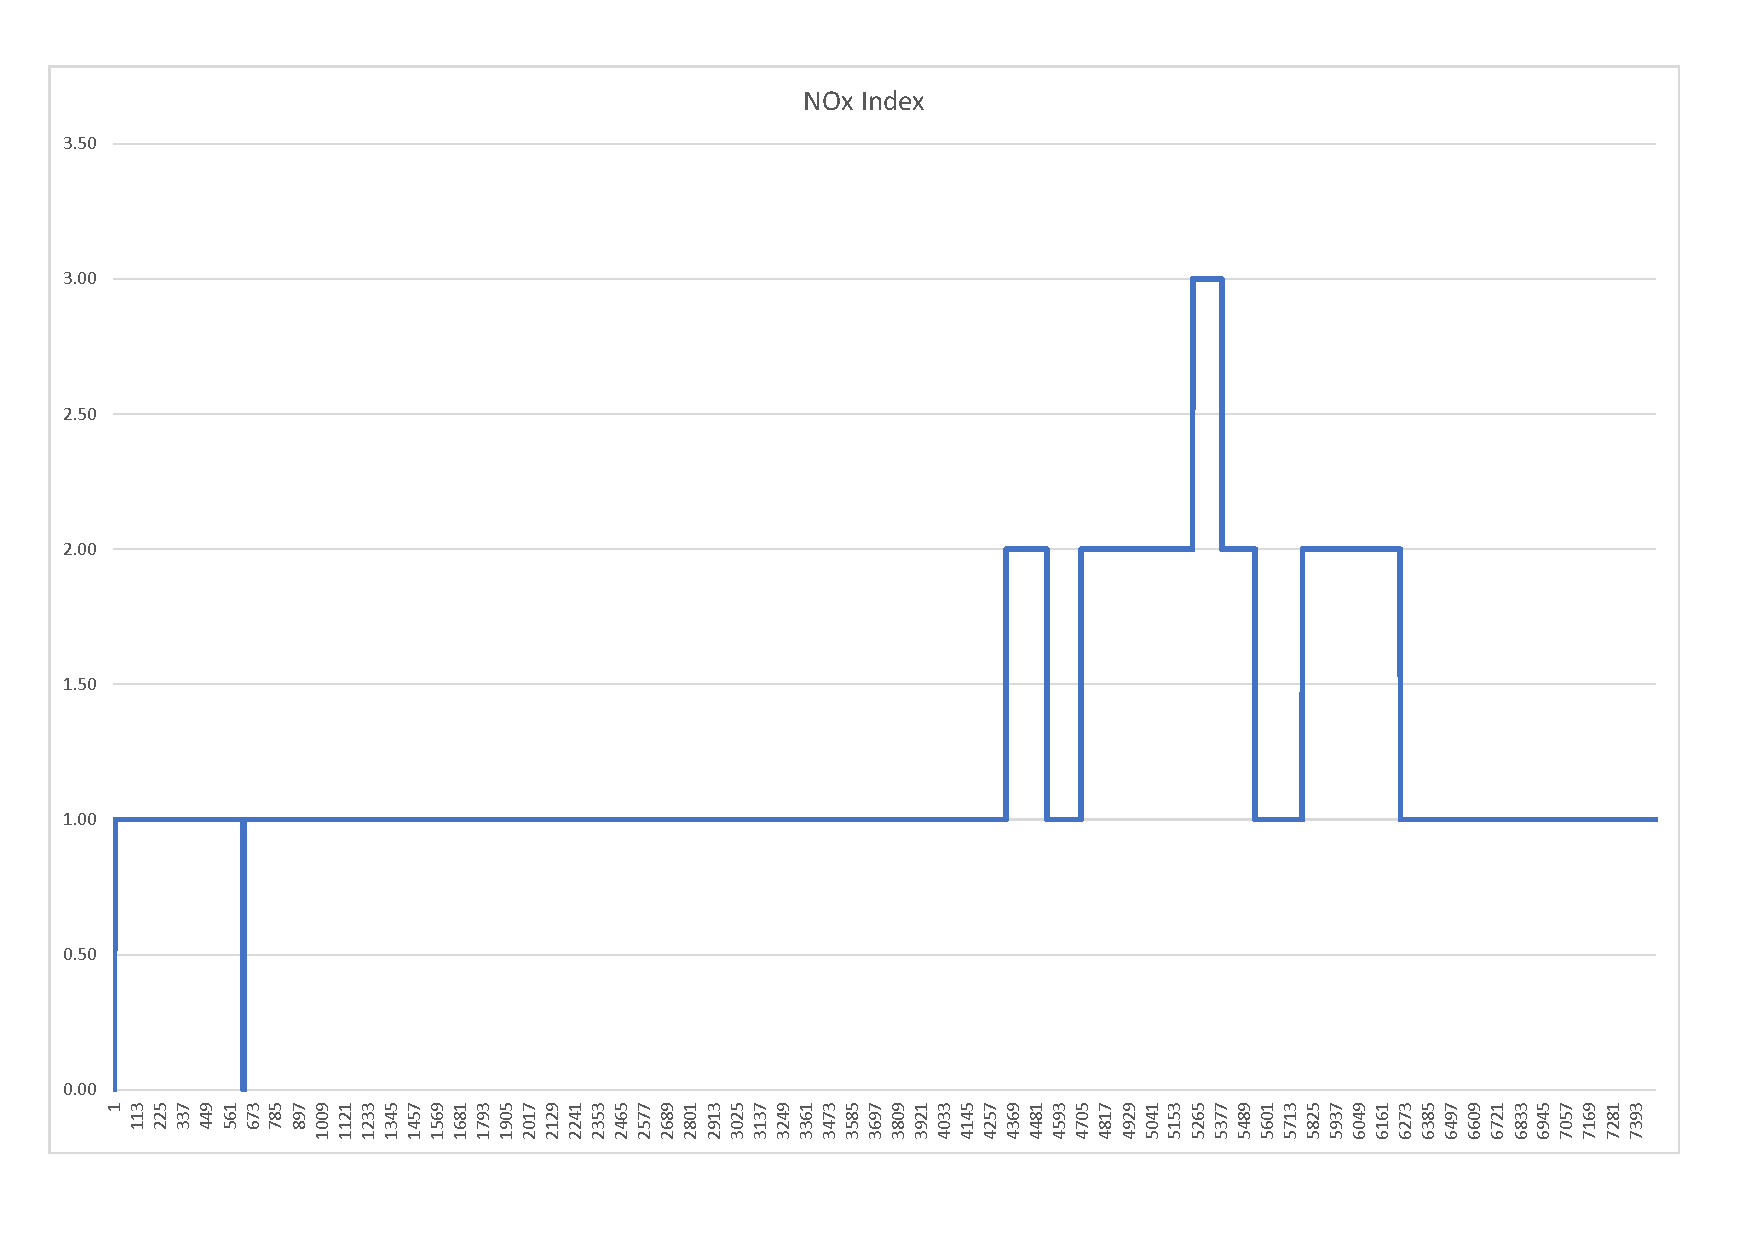
\includegraphics[width=0.5\textwidth]{body/fig/NOX.pdf}%
%	\captionof{figure}{Humidity}
%	\label{fig:nox}
%\end{figure}
\begin{figure}[!htb]
	\minipage{0.45\textwidth}%
	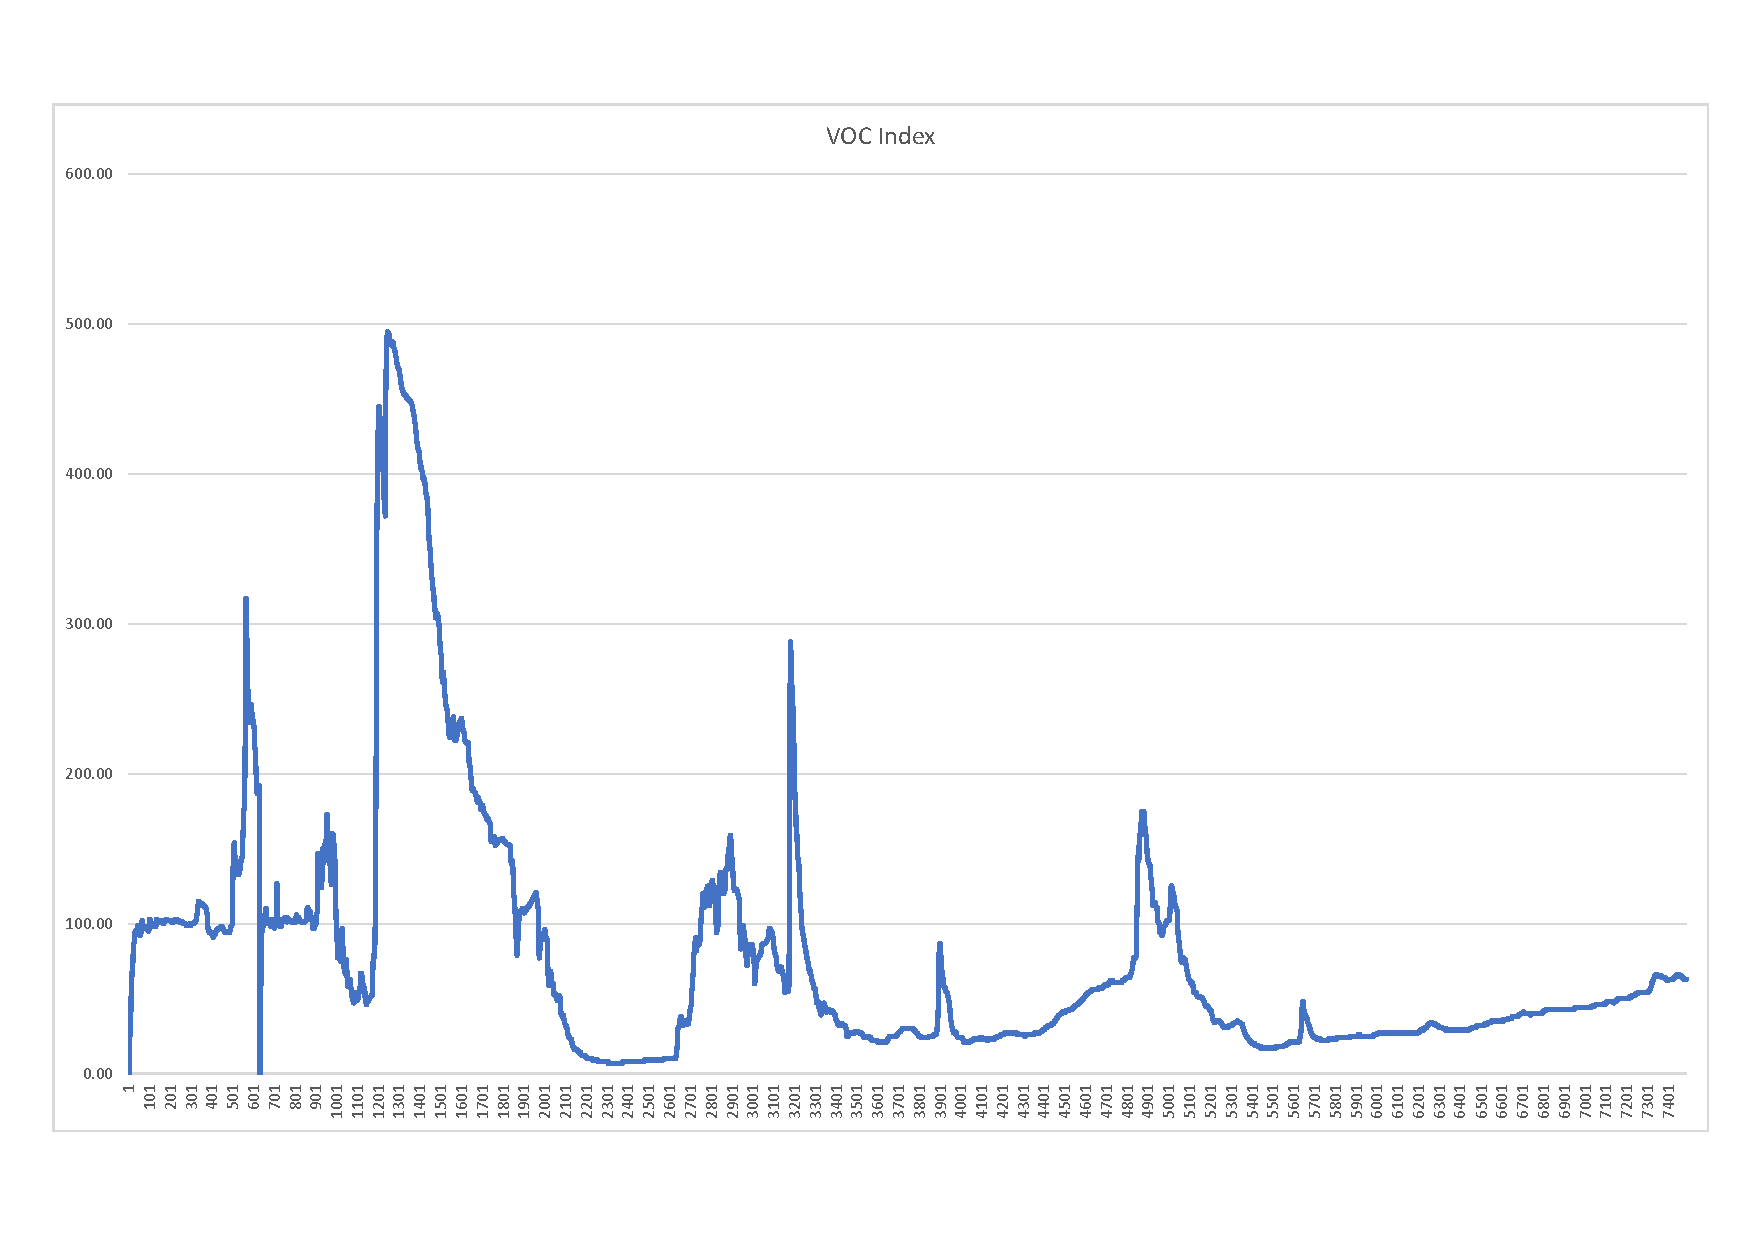
\includegraphics[width=\linewidth]{body/fig/VOC.pdf}
	\caption{VOC}\label{fig:voc}
	\endminipage\hfill
	\minipage{0.45\textwidth}%
	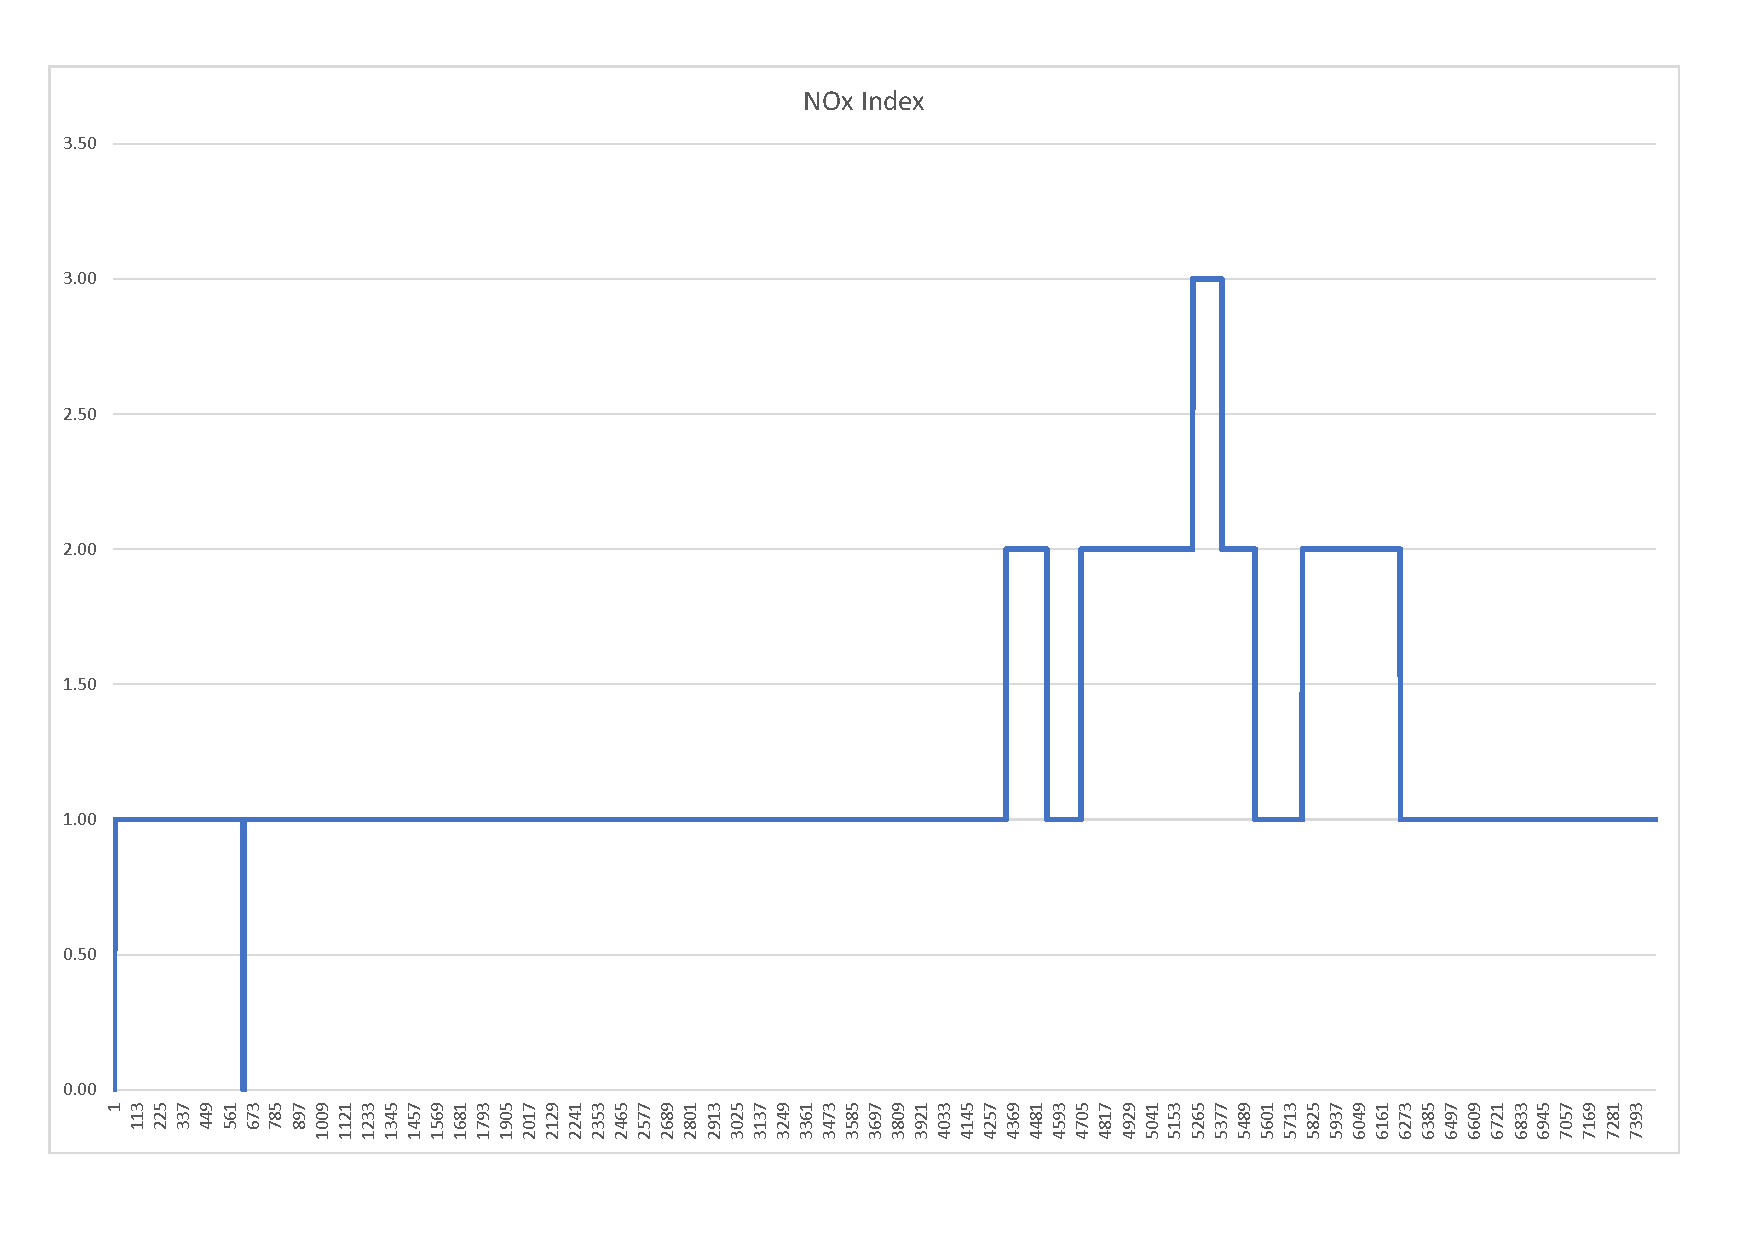
\includegraphics[width=\linewidth]{body/fig/NOX.pdf}
	\caption{NOx}\label{fig:nox}
	\endminipage\hfill

	%\text{Charts provided by \cite{2007Comparison}}
\end{figure}

